%Implementierung_dotmul

\subsubsection{dotmul}

Im Bild \ref{Vektor} wird das Implementierungsmethode in CUDA gezeigt. A und B sind Vektoren, die sich miteinander in jeweiligem Thread multipliziert werden müssen. Cs sind erzeugte Produktvektoren, die allen zu einem Wert summiert werden. Da eine Beschrankung des CUDA-Blocksizes maximum 512 Threads enthält, muss ein Block iterativ oder mehrere Blocks verwendet werden.

\begin{figure}[htbp]
%\centering
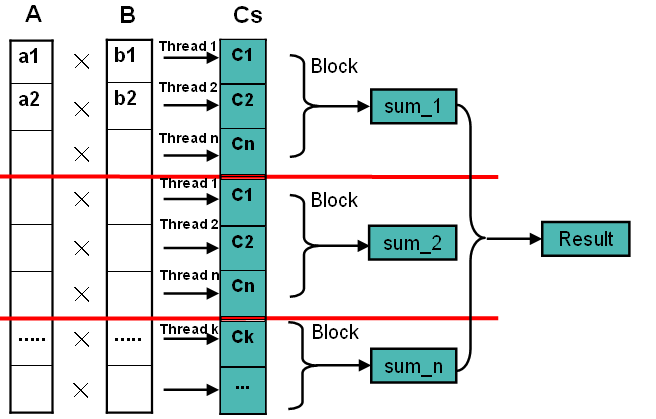
\includegraphics[width=3.5in]{../xby/pic/Vektor}
\caption{Vektor Multiplikation. A : Erst Vektor; B: Zweiter Vektor; Cs: Produktvektor}
\label{Vektor}
\end{figure}